\documentclass[msc,lith,english]{liuthesis}

%%%%%%%%%%%%%%%%%%%%%%%%%%%%%%%%%%%%%%%%%%%%%%%%%
% Imports
%%%%%%%%%%%%%%%%%%%%%%%%%%%%%%%%%%%%%%%%%%%%%%%%%
%\usepackage[english]{babel}
\usepackage[utf8]{inputenc}
\usepackage[backend=biber,sorting=none,hyperref]{biblatex}
\usepackage{mathtools}
\usepackage{dsfont}
\usepackage{tikz}
\usetikzlibrary{topaths,calc,tikzmark}
\usepackage{algorithm2e}
\usepackage{pgfgantt}

%%%%%%%%%%%%%%%%%%%%%%%%%%%%%%%%%%%%%%%%%%%%%%%%%
% Settings
%%%%%%%%%%%%%%%%%%%%%%%%%%%%%%%%%%%%%%%%%%%%%%%%%
\department{TODO:DEPARTMENT}
\departmentenglish{TODO:DEPARTMENT}
\departmentshort{ISY}

\supervisor{Frans Skarman}
\examiner{TODO:DANIEL SOMETHING
\titleenglish{}
% \subtitleenglish{100\% rainbow-free guarantee}
\titleswedish{}
\thesissubject{Datateknik}

\publicationyear{2023}
\currentyearthesisnumber{001}
\dateofpublication{2023-05-20}

\addbibresource{thesis.bib}

\newcommand\tikznode[3][]%
   {\tikz[remember picture, baseline=(#2.base)]
      \node[minimum size=0pt,inner sep=0pt,#1](#2){#3};%
   }

\author{Edvard Thörnros}

\begin{document}

%%%%%%%%%%%%%%%%%%%%%%%%%%%%%%%%%%%%%%%%%%%%%%%%%
% Intro
%%%%%%%%%%%%%%%%%%%%%%%%%%%%%%%%%%%%%%%%%%%%%%%%%
\chapter{Introduction}
\label{chaIntro}

\section{Research questions}
\begin{enumerate}
  \item A
  \item B
\end{enumerate}
*Speed is defined by asymptotic computational complexity.

\section{Aim}

\section{Delimitations}

%%%%%%%%%%%%%%%%%%%%%%%%%%%%%%%%%%%%%%%%%%%%%%%%%
% Background
%%%%%%%%%%%%%%%%%%%%%%%%%%%%%%%%%%%%%%%%%%%%%%%%%
\chapter{Background}
\label{chaBackground}

\section{Graphs}

\chapter{Related Work}

\section{Exact Algorithms for No-Rainbow Coloring and Phylogenetic Decisiveness}

\chapter{Project Plan}

\section{Method}

\section{Expected Results}

\section{GANTT-chart}
A GANTT-chart of the work is presented in Figure \ref{figGanttChart}.

\begin{center}
\begin{figure}[htp]
\begin{ganttchart}[
    vgrid,
    bar left shift=0.15,
    bar right shift=-0.15,
    bar/.append style={rounded corners=3pt},
    bar inline label node/.style={%
      anchor=south, font=\ganttvalueof{bar label font}%
    },%
    inline,
    milestone inline label node/.style={%
      anchor=north, font=\ganttvalueof{milestone label font}%
    },%
    expand chart=\textwidth
]{1}{20}
\gantttitle{Project Plan}{20} \\
\gantttitlelist{1,...,20}{1} \\

\ganttgroup{Problem}{1}{13} \\
\ganttbar{Discover solutions}{1}{9}
\ganttlinkedbar{Present solution}{10}{13} \\
\ganttmilestone{Show to examiner}{4}
\ganttmilestone[milestone inline label node/.style={anchor=south}]{Solution OK by examiner}{9} \\
\\
\ganttgroup{Report}{1}{19} \\
\ganttbar{Related works}{2}{8} \\
\ganttbar{Discussion}{11}{13} \\
\ganttbar{Conclusion}{14}{14} \\
\ganttbar{Introduction}{15}{15} \\

\ganttbar{Polish report}{16}{17} \\
\ganttlinkedbar{Presentation}{18}{20} \\

\ganttmilestone{Find opponent}{16} \\
\ganttmilestone{1st hand in}{17} \\

\ganttmilestone[milestone inline label node/.style={anchor=north east}]{Hold presentation and final hand in}{20} \\

\ganttlink{elem1}{elem7}
\ganttlink{elem7}{elem8}
\ganttlink{elem6}{elem7}
\ganttlink{elem8}{elem9}
\ganttlink{elem9}{elem10}
\end{ganttchart}
  \caption{The project plan for the final thesis.}
  \label{figGanttChart}
\end{figure}
\end{center}

\subsection{Polish report}
In the report group, each task corresponds to a chapter except ``Polish report``.
The ``Polish report`` chapter is for fixing everything else that needs fixing.
The vague heading ``Polish report`` will also serve as slack for the project.

\subsection{Related works}
The goal with ``related works`` is to write the related works section and understand the subject in a wider context.
This activity results in a finished background/related works section, and a broader understanding of the subject.
Both the background and related works should preferably be too large here to be trimmed later.

\subsection{Discussion}
The discussion is written here.

\subsection{Conclusion}
The conclusion is written here.

\subsection{Introduction}
The Introduction is written here.

\subsection{Discover solutions}
The heading ``Discover solutions`` also needs some clarification. Constructing
an algorithm is a creative process. For a creative process it is instrumental
to move between working and thinking. The related works section is scheduled for
parts of the duration of discovering solutions. Since knowing more about the
area will feed back into new ideas for other algorithmic solutions. 
Figure \ref{figCreativeProcess} contains a visualization of the workflow I imagine.

\begin{center}
\begin{figure}[h!]
\centering
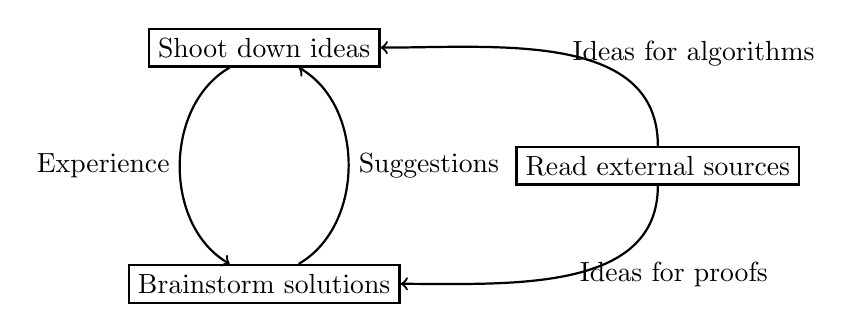
\begin{tikzpicture}[thick, node/.style = {draw}]
  \node[node] (a) at (0,0) {Brainstorm solutions};
  \node[node] (b) at (0,3) {Shoot down ideas};
  \node[node] (c) at (5,1.5) {Read external sources};

  \draw[->] (a) to[out=30,in=-30] node[right]{Suggestions} (b);
  \draw[->] (b) to[out=-150,in=150] node[left]{Experience} (a);
  \draw[->] (c) to[out=-90,in=0] node[right]{Ideas for proofs} (a);
  \draw[->] (c) to[out=90,in=0] node[right]{Ideas for algorithms} (b);
\end{tikzpicture}
\caption{The creative process of constructing algorithms according to the author.}
\label{figCreativeProcess}
\end{figure}
\end{center}

\subsection{Present solution}
Extra work is put into presenting the solution and writing a solid proof.
This means polishing the proof to make the proofs as clear and well written as possible.
Here the bulk of the report is written.
The proofs and the explanations are put into place as the basis for the rest of the thesis.

\subsection{Milestones ``Show to examiner`` and ``Solution OK by examiner``}
These milestones will give me deadline.
These deadlines stop the creative process of discovering algorithms from losing focus.
I will know if these milestones are reached if my examiner thinks the work is good.
The `Solution OK by examiner`` correspond to the halftime reviews.

\subsection{Milestone ``Find opponent``}
Will find someone to oppose me, and preferably someone to oppose. 

\subsection{Milestone ``1st hand in``}
A first version of the thesis is handed in, in a state that I would be happy to
publish. But expecting further revisions.

\subsection{Milestone ``Hold presentation and final hand in``}
The final presentation is held. I get feedback from my examiner and my
opponent. This feedback is the quickly revised then the thesis can be sent for
publishing.

\section{Risks}

\begin{enumerate}
  \item (\textbf{likelihood:} medium, \textbf{severity:} high)
    The largest risk for failure is if no sufficiently good algorithm
    is found the project will have to be restructured. Either a different problem
    will have to be chosen (preferably in a related area), or the thesis will have
    to pivot to focus more on why there is not a faster algorithm.

  \item (\textbf{likelihood:} low, \textbf{severity:} medium)
    The examiner might not know enough about the subject area to give valid
    guidance. This might prolong the project and force me to redo work. I will
    have to be critical of the feedback from my examiner and make sure I have a
    solid understanding.

  \item (\textbf{likelihood:} medium, \textbf{severity:} low)
    There might not be enough background surrounding the no-rainbow problem.
    This will force me to branch out more in my research but should still allow
    me to formulate a good thesis. The project might take more time if there
    are few sources. To mitigate this I should read a wide variety of articles.
\end{enumerate}

\printbibliography
